\section{Introduction}
% In the coming many-core era, due to the tight power budget, power efficiency is cricital for multi-core chip design. In the previous work by Dong Hyuk Woo, evaluation of energy efficiency on the basis of performance and power (PPW) models is developed, which shows the tendency of PPW with number of cores. However, due to the dependency of leakage current on temperature and the prevalence of DVFS and dark silicon in multicore processor, the speedup potential given by existing extending methods of Amdahl's law no longer works out. In this paper, We implement dark silicon and thermal model into the evaluation of PPW to provide an alternative suitable with the dark silicon era.

Integrated circuit (IC) has been through the most remarkable technology advances in the past few decades, thanks to the constant exponential increase of IC integration density in the meanwhile, which is described by the famous Moore's law. However, with the failure of Dennard scaling, power density begins to rise with integration density, resulting in serious thermal related problems in IC systems. Especially in recent years, power density has increased beyond the power wall caused by limited heat dissipation capability of the chip, leading to the fact that not all components of the systems can be activated or run at full speed at the same time. Such system is called dark silicon system or system in dark silicon~\cite{Hardavellas:MICRO'11,Goulding-Hotta:MICRO'11,Esmaeilzadeh:MICRO'12,Taylor:DAC'12,Taylor:MICRO'13,WangMa:TODAES'16}.

Nowadays, multi-core systems have become the main stream of computing systems. For multi-core systems in dark silicon, a fundamental problem is to control the operation of each of the individual cores to maximize certain objective. Depending on the objective, the voltage and frequency levels (VF levels) of the active cores can be adjusted, and tasks can be scheduled according to the active core number and their VF levels, while the constraints on power consumption and temperature have to be satisfied. Typically when the objective is the performance of the multi-core system in dark silicon, the constraints on power consumption is the maximum allowed power, which should never be exceeded to avoid thermal emergencies. Such maximum allowed power is called power budget, and the process of finding it is called the power budgeting process. 

%Many researches have been done on solving the power budget issues of dark silicon systems. Such as.

However, the maximum performance and the maximum energy efficiency of a system generally cannot be achieved at the same time. Fig.~\ref{fig:ppw_mips} shows the result of simulating the execution of a set of benchmark programs on a single core of a $16$-core system, and tracking the ratio of the throughput to energy as the throughput of the core varies. The ratio is a measure of energy efficiency and is referred to as performance-per-watt (PPW), which is equivalent to the number of instructions executed per Joule of energy. As the figure shows, the PPW has a unique maximum value when the throughput is $31$ MIPS, which means that the power budget that maximizes the energy-efficiency of the system differs from the ones of maximum performance of worst performance of the system. Hence, a power budgeting method that can provide optimal energy efficiency is strongly needed.



\begin{figure}
\centering
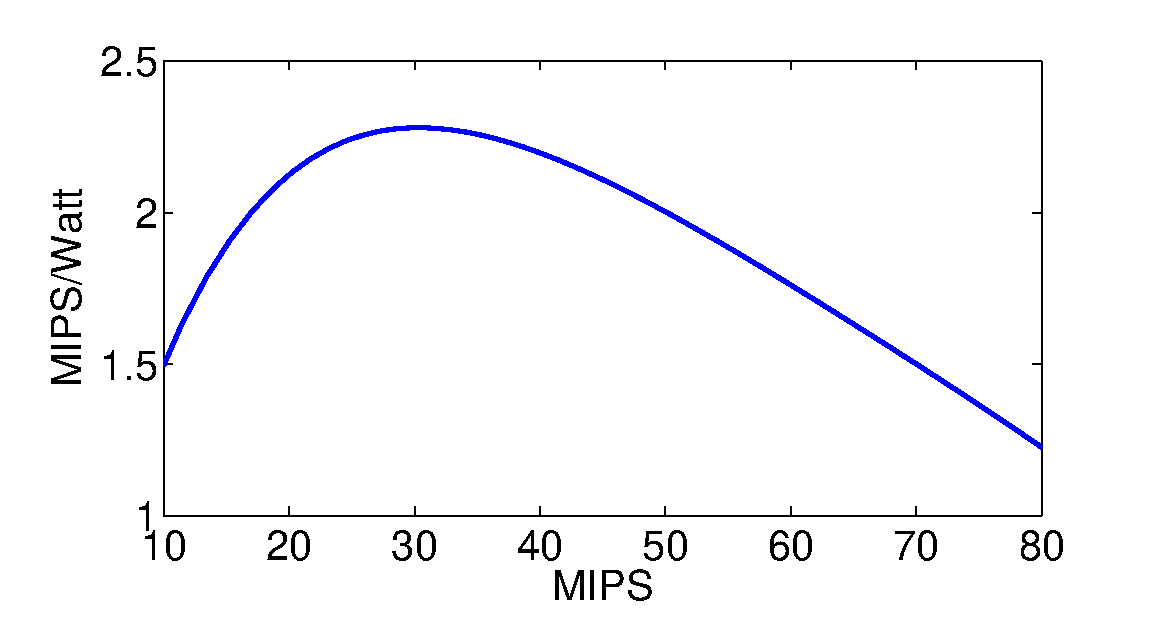
\includegraphics[width=1\linewidth]{fig/ppw_mips.eps}
\caption{MIPS/Watt-MIPS curve of turning on a single core in steady state, where a unique maximum value of MIPS/Watt with the corresponding MIPS $=31$ exists.}
\label{fig:ppw_mips}
\end{figure}

In this work, we propose a fast power budgeting method which can maximize the PPW of a homogeneous multi-core system in dark silicon while the power budget remaining as high as possible. This work formulates the power budgeting problem as thermal-constrained combinational optimization problem. To speed up the solution of the problem, we invoke two new ideas: first, we transform the original PPW-optimization problems to an easier solving temperature-optimization problem; second, since the power budget varies with the locations of the active cores for dark silicon systems, a greedy based method to find the sub-optimal active core distribution which maximizes power budget, and computes its corresponding power budget at runtime.

The remaining part of this article is organized as follows. First, we review related work in power budgeting of IC systems and present the motivation of this work in Section 2. Then the modeling of the multi-core packaged IC system is introduced in Section 3, which serves as prerequisite knowledge for power budgeting. In section 4, the energy-efficient dynamic power budgeting method is presented. Next, experiments implemented to verify the effectiveness and analyze the performance of the new method are demonstrated in Section 5. Conclusion is drawn in Section 6.